\documentclass[9pt,a4paper]{report}
\usepackage{amsfonts,amsmath,amsthm,amssymb,graphicx,graphics}
\usepackage{indentfirst,tikz,wrapfig,caption,multirow}
\usepackage[utf8x]{inputenc}
\renewcommand\figurename{Figura}
\renewcommand\chaptername{Capitolul}
\renewcommand\bibname{Bibliografie}
\newtheorem{definitie}{Definiția}
\newtheorem{teorema}{Teorema}

\title{\bf Introducere în teoria grafurilor}
\author{Sîrbu Matei-Dan}
\date{decembrie 2020}

\begin{document}
\maketitle

\newpage

\chapter{Despre conceptul de \textit{graf}}
\section{Terminologie}

Definim în mod informal un graf ca fiind o colecție de ,,noduri'' unite prin ,,muchii'', ca în exemplul următor:

\begin{figure}[htbp]
    \centering
    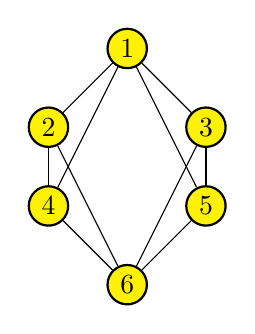
\begin{tikzpicture}[every node/.style={draw=black,thick,circle,inner sep=0pt,fill=yellow,minimum size=0.5cm}]
        \node[] (1) at (0,0) {1};
        \node[] (2) at (-1,-1) {2};
        \node[] (3) at (1,-1) {3};
        \node[] (4) at (-1,-2) {4};
        \node[] (5) at (1,-2) {5};
        \node[] (6) at (0,-3) {6};

        \path [-] (1) edge (3);
        \path [-] (1) edge (4);
        \path [-] (1) edge (5);
        \path [-] (2) edge (4);
        \path [-] (1) edge (2);
        \path [-] (2) edge (6);
        \path [-] (3) edge (5);
        \path [-] (3) edge (6);
        \path [-] (4) edge (6);
        \path [-] (5) edge (6);
    \end{tikzpicture}
    \caption{Un graf neorientat oarecare.}
    \label{fig:graf1}
\end{figure}

\begin{definitie}
    Un \textbf{graf} este o pereche $(V,E)$, unde $V$ este o mulțime finită de elemente, numite \textit{noduri (\textbf{V}ertices)}, iar $E$ este o mulțime finită de perechi de noduri, numite \textit{muchii (\textbf{E}dges)}.
\end{definitie}

Dacă perechile din mulțimea $E$ sunt ordonate, atunci spunem că graful este \textbf{\textit{orientat}}, sau \textbf{\textit{digraf}}; în caz contrar, graful este \textbf{\textit{neorientat}}. De asemenea, două noduri unite de o muchie se numesc \textit{\textbf{adiacente}}. Conceptul analog muchiilor aplicabil grafurilor orientate este \textbf{\textit{arcul}}.

\section{Dimensiunile unui graf}

De obicei, notăm cu $n$ numărul de noduri ale unui graf; mai precis, $n = |V|$. Cu $m$ vom nota numărul de muchii, adică $m = |E|$. În graful din figura \ref{fig:graf1}, $n$ este 6, iar $m$ este 10.

\begin{teorema}
    Dacă un graf neorientat are $n$ noduri, atunci \textbf{\textit{numărul total de grafuri neorientate}} care se pot forma cu aceste noduri este $g = 2^{C_n^2}$.
\end{teorema}

\begin{teorema}
    Graful \textbf{\textit{complet}}, graful care are toate muchiile posibile, conține $m = \frac{n(n-1)}{2}$ muchii, dacă este neorientat.
\end{teorema}

Spunem despre un nod că este \textbf{\textit{izolat}} dacă nu aparține niciunei muchii. Întrucât nodurile izolate sunt inutile în majoritatea aplicațiilor, presupunem că nu există astfel de noduri; în acest caz, știm despre numărul de muchii că este $m \geq \frac{n}{2}$.

Astfel, deducem, utilizând simbolul O al lui Landau (notația \textit{big-O}), că în general, $m = O(n^2)$, iar în majoritatea aplicațiilor, $m = \Omega(n)$, limite care sunt aplicabile și digrafurilor. Din punct de vedere terminologic, grafurile cu $m = \Theta(n)$ se numesc \textbf{\textit{rare}}, iar cele cu $m = \Theta(n^2)$ sunt \textbf{\textit{dense}}.

\section{Conexitate}

\begin{definitie}
    Un \textbf{subgraf} $G' = (V', E')$ este un subgraf al lui $G = (V, E)$ dacă $V' \subseteq V$ și $E' \subseteq E$.
\end{definitie}
\begin{definitie}
    Un \textbf{lanț} este o succesiune de noduri $v_0, v_1, \dots, v_l$, $l \geq 0$, cu $(v_i, v_{i+1}) \in E$ pentru $i = \overline{0, \ l - 1}$. Analog, în cazul grafurilor orientate, această succesiune de noduri se numește \textbf{drum}.
\end{definitie}

Un lanț este \textbf{\textit{simplu}} dacă nu trece de două ori prin aceeași muchie. În caz contrar, se numește lanț \textbf{\textit{compus}}. Este de remarcat faptul că un lanț poate avea lungime nulă.

\begin{definitie}
    Un \textbf{ciclu} este un drum cu $l \geq 3$, $v_0 = v_l$ cu toate nodurile și muchiile distincte.
\end{definitie}

\begin{thebibliography}{9}
    \bibitem{gabow} 
    Harold N. Gabow. 
    \textit{Graph Theory Definitions}. 
    The Department of Computer Science at the University of Colorado Boulder, 2008.
    
    \bibitem{milosescu} 
    Mariana Miloșescu. 
    \textit{Informatică intensiv: C++: manual pentru clasa a XI-a, ed. a 3-a}.
    Editura Didactică și Pedagogică, 2012.
    
    \end{thebibliography}

\end{document} 